\documentclass[tikz,border=4pt]{standalone}
\usepackage{amsmath}
\usetikzlibrary{arrows.meta,positioning}
\begin{document}
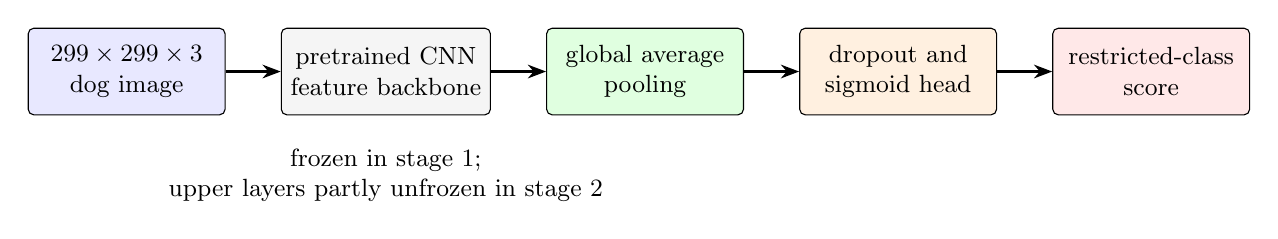
\begin{tikzpicture}[
  >=Stealth,
  node distance=7mm,
  every node/.style={font=\small},
  stage/.style={draw,rounded corners=2pt,minimum height=11mm,minimum width=25mm,align=center},
  arrow/.style={->,thick}
]
  \node[stage,fill=blue!9] (image) {$299\times299\times3$\\dog image};
  \node[stage,fill=gray!8,right=of image] (cnn) {pretrained CNN\\feature backbone};
  \node[stage,fill=green!12,right=of cnn] (pool) {global average\\pooling};
  \node[stage,fill=orange!12,right=of pool] (head) {dropout and\\sigmoid head};
  \node[stage,fill=red!9,right=of head] (score) {restricted-class\\score};
  \draw[arrow] (image) -- (cnn);
  \draw[arrow] (cnn) -- (pool);
  \draw[arrow] (pool) -- (head);
  \draw[arrow] (head) -- (score);
  \node[below=3mm of cnn,align=center] {frozen in stage 1;\\upper layers partly unfrozen in stage 2};
\end{tikzpicture}
\end{document}
